\documentclass[border=10pt]{standalone}
\usepackage[svgnames]{xcolor}
\usepackage{amsmath}
\usepackage{pgfplots}
\pgfplotsset{compat=newest}
\usepackage[sfdefault]{FiraSans}
\usepackage{FiraMono}
\renewcommand*\familydefault{\sfdefault}
\begin{document}
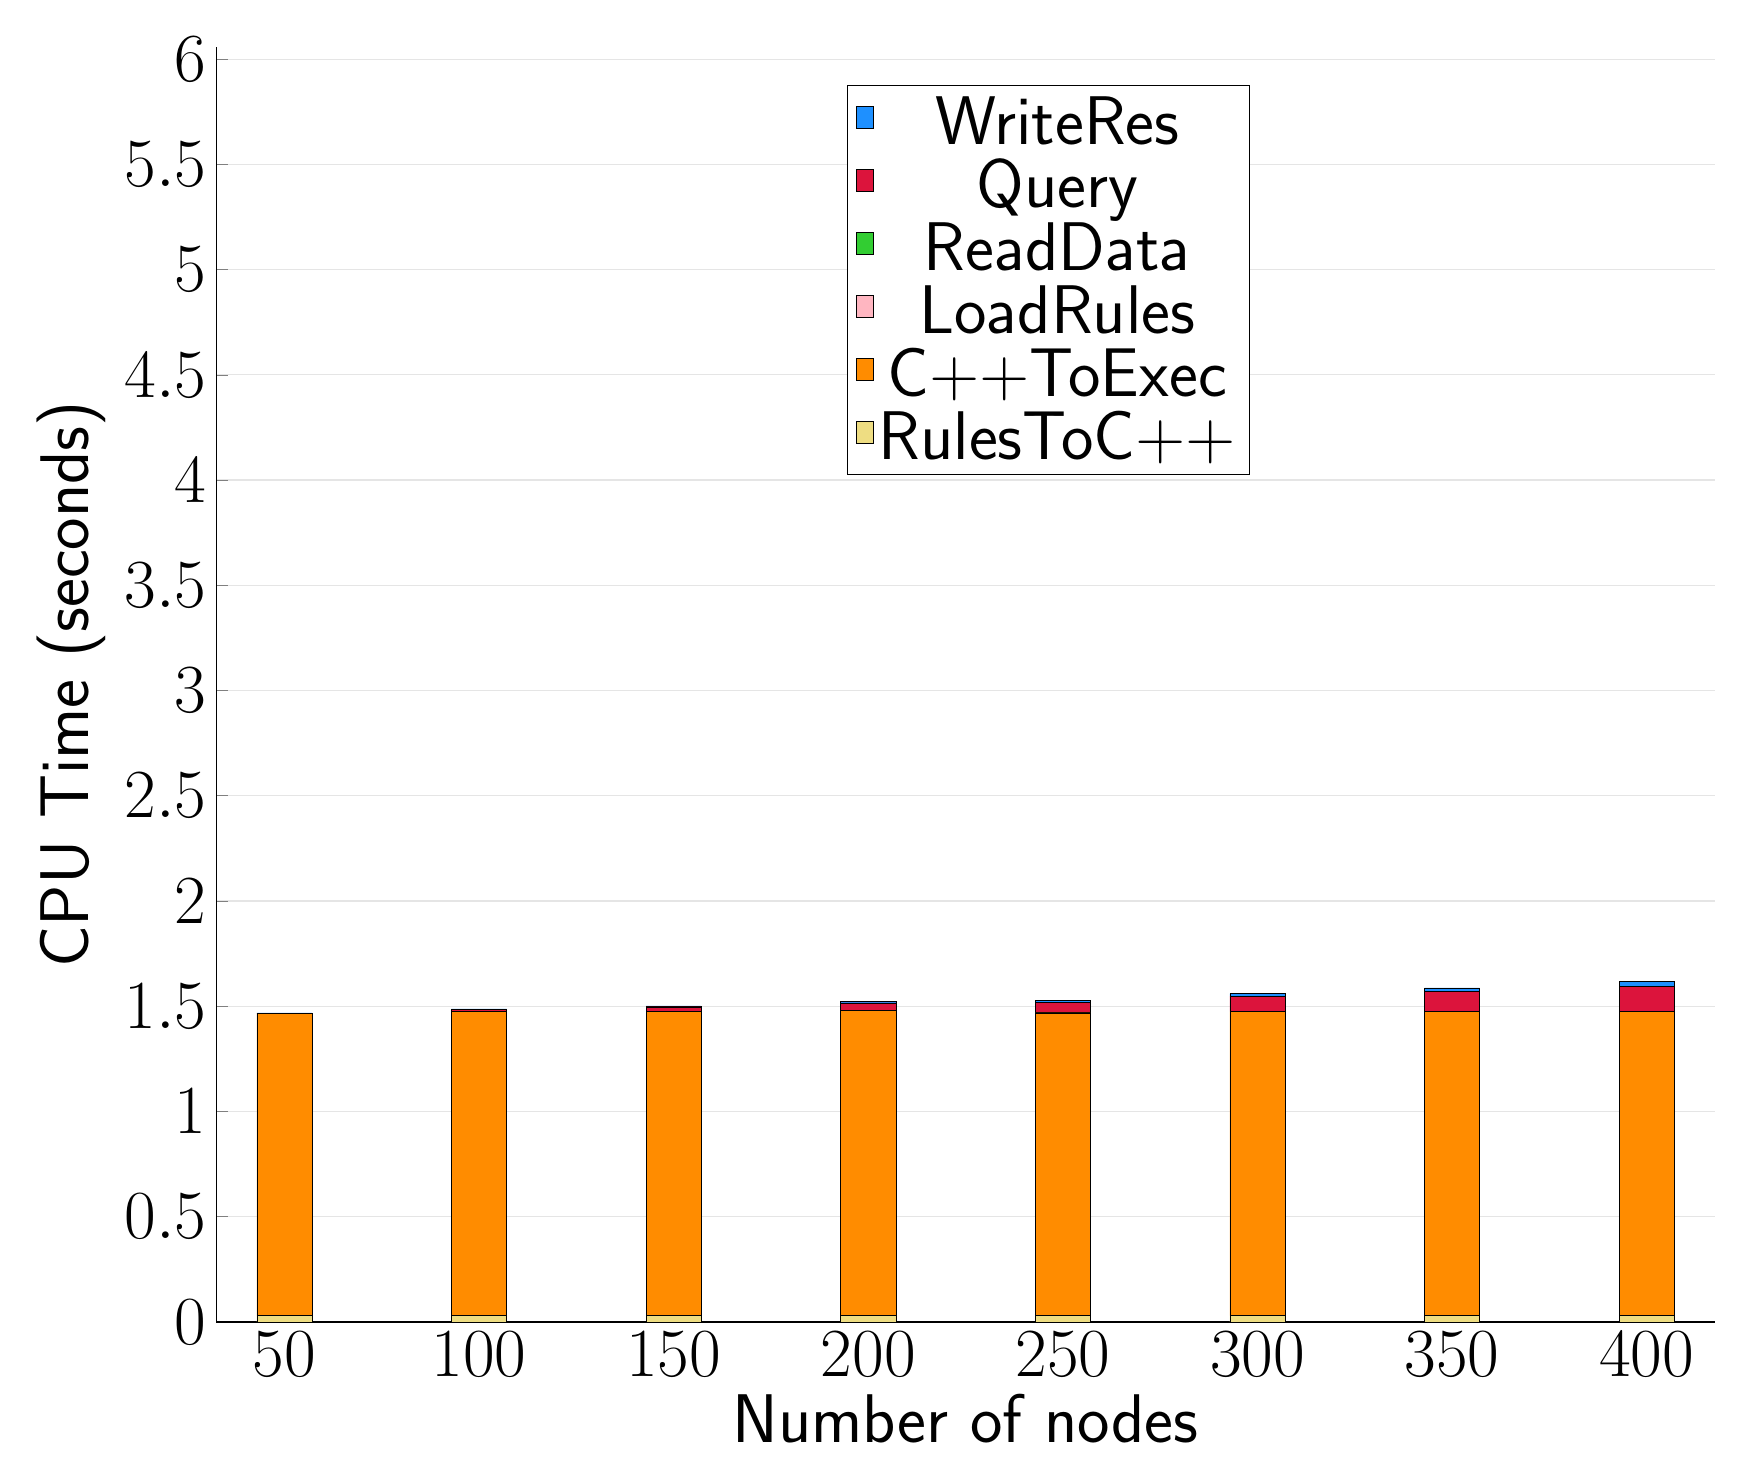
\begin{tikzpicture}
	\begin{axis}[
			ybar stacked,
			width=1.7\textwidth,
			bar width=0.7cm,
			ymajorgrids, tick align=inside,
			major grid style={draw=gray!20},
			xtick=data,
			ymin=0, ymax=6.059334,
			axis x line*=bottom,
			axis y line*=left,
			enlarge x limits=0.05,
			legend style={
					at={(0.69, 0.97)},
					anchor=north east,
					legend columns=1,
					font=\Huge,
				},
			ylabel={CPU Time (seconds)},
			xlabel={Number of nodes},
			label style={font=\Huge},
			tick label style={font=\Huge},
		]
		\addlegendimage{fill=DodgerBlue, draw=black, line width=0.2pt}
		\addlegendentry{WriteRes}
		\addlegendimage{fill=Crimson, draw=black, line width=0.2pt}
		\addlegendentry{Query}
		\addlegendimage{fill=LimeGreen, draw=black, line width=0.2pt}
		\addlegendentry{ReadData}
		\addlegendimage{fill=LightPink, draw=black, line width=0.2pt}
		\addlegendentry{LoadRules}
		\addlegendimage{fill=DarkOrange, draw=black, line width=0.2pt}
		\addlegendentry{C++ToExec}
		\addlegendimage{fill=LightGoldenrod, draw=black, line width=0.2pt}
		\addlegendentry{RulesToC++}
		\addplot +[fill=LightGoldenrod, draw=black, line width=0.2pt] coordinates {
				(50, 0.030000000000000006)
				(100, 0.031)
				(150, 0.030000000000000006)
				(200, 0.030000000000000006)
				(250, 0.030000000000000006)
				(300, 0.030000000000000006)
				(350, 0.030000000000000006)
				(400, 0.030000000000000006)
			};
		\addplot +[fill=DarkOrange, draw=black, line width=0.2pt] coordinates {
				(50, 1.4349999999999998)
				(100, 1.4449999999999998)
				(150, 1.4459999999999997)
				(200, 1.4499999999999997)
				(250, 1.4389999999999996)
				(300, 1.4449999999999996)
				(350, 1.4439999999999995)
				(400, 1.4449999999999996)
			};
		\addplot +[fill=LightPink, draw=black, line width=0.2pt] coordinates {
				(50, 1.11e-05)
				(100, 1.1e-05)
				(150, 0.0)
				(200, 1.1e-05)
				(250, 0.0)
				(300, 0.0)
				(350, 1.1e-05)
				(400, 2.14e-05)
			};
		\addplot +[fill=LimeGreen, draw=black, line width=0.2pt] coordinates {
				(50, 0.000411)
				(100, 0.0004953999999999999)
				(150, 0.0006119999999999999)
				(200, 0.0007427)
				(250, 0.0007319999999999999)
				(300, 0.0009214)
				(350, 0.0010491)
				(400, 0.0010789)
			};
		\addplot +[fill=Crimson, draw=black, line width=0.2pt] coordinates {
				(50, 0.0021315999999999996)
				(100, 0.009199599999999999)
				(150, 0.020832)
				(200, 0.03505219999999999)
				(250, 0.049353999999999995)
				(300, 0.0719398)
				(350, 0.09511539999999999)
				(400, 0.1196245)
			};
		\addplot +[fill=DodgerBlue, draw=black, line width=0.2pt] coordinates {
				(50, 0.0007411000000000001)
				(100, 0.0021907)
				(150, 0.0043235)
				(200, 0.006561699999999999)
				(250, 0.009152799999999999)
				(300, 0.012706899999999998)
				(350, 0.0170911)
				(400, 0.0223557)
			};
	\end{axis}
\end{tikzpicture}

\end{document}
